\documentclass[aspectratio=169]{beamer}
\usetheme{Madrid}
\usepackage[utf8]{inputenc}
\usepackage{graphicx}
\usepackage{amsmath}
\usepackage{booktabs}
\usepackage{tikz}
\usetikzlibrary{arrows.meta,positioning,shapes,fit,calc}

% App-like dark theme colors
\newif\iflighttheme
\lightthemetrue

\definecolor{slate900}{HTML}{0F172A}
\definecolor{slate800}{HTML}{1E293B}
\definecolor{slate700}{HTML}{334155}
\definecolor{slate200}{HTML}{E2E8F0}
\definecolor{slate100}{HTML}{F8FAFC}
\definecolor{cyan400}{HTML}{22D3EE}
\definecolor{indigo400}{HTML}{818CF8}

\iflighttheme
  \setbeamercolor{background canvas}{bg=slate100}
  \setbeamercolor{normal text}{fg=slate900}
  \setbeamercolor{frametitle}{fg=slate900,bg=slate200}
  \setbeamercolor{title}{fg=slate900}
  \setbeamercolor{subtitle}{fg=slate800}
  \setbeamercolor{structure}{fg=indigo400}
\else
  \setbeamercolor{background canvas}{bg=slate900}
  \setbeamercolor{normal text}{fg=slate100}
  \setbeamercolor{frametitle}{fg=slate100,bg=slate800}
  \setbeamercolor{title}{fg=slate100}
  \setbeamercolor{subtitle}{fg=slate100}
  \setbeamercolor{structure}{fg=cyan400}
\fi
\setbeamertemplate{navigation symbols}{}

\title{GeoAuPredict: Diagrams}
\subtitle{Auto-generated TikZ inputs}
\author{GeoAuPredict Team}
\date{\today}

\begin{document}

\frame{\titlepage}

\begin{frame}{End-to-End Pipeline Flow}
\centering
% This file is generated by generate_diagrams.py
\resizebox{!}{0.78\textheight}{
% Auto-generated by generate_diagrams.py
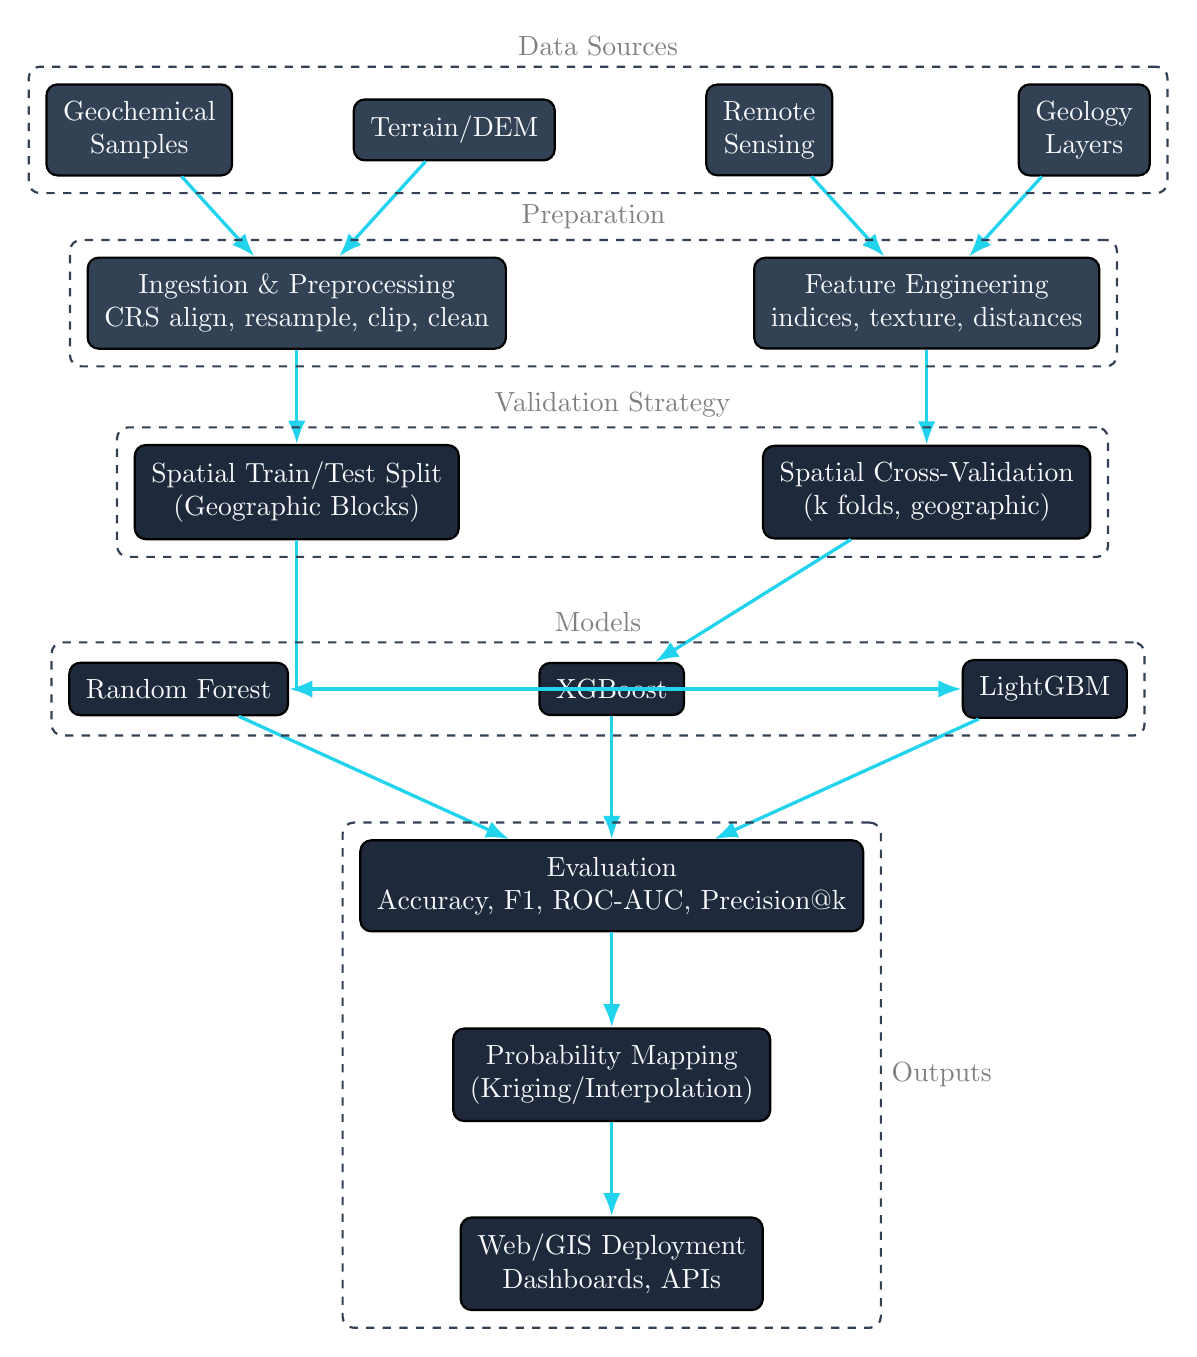
\begin{tikzpicture}[node distance=1.6cm]
  % Styles
  \tikzset{
    block/.style={draw, rounded corners, thick, align=center, fill=slate800, text=slate100, inner sep=6pt},
    data/.style={draw, rounded corners, thick, align=center, fill=slate700, text=slate100, inner sep=6pt},
    process/.style={draw, rounded corners, thick, align=center, fill=slate700, text=slate100, inner sep=6pt},
    result/.style={draw, rounded corners, thick, align=center, fill=slate800, text=slate100, inner sep=6pt},
    dashedblock/.style={draw=slate700, rounded corners, thick, align=center, dashed, inner sep=6pt},
    line/.style={-Latex, very thick, draw=cyan400},
  }

  % Row 1: Data sources (explicit coordinates to avoid overlap)
  \node[data] (geochem) at (0,0) {Geochemical\\Samples};
  \node[data] (terrain) at (4,0) {Terrain/DEM};
  \node[data] (remote)  at (8,0) {Remote\\Sensing};
  \node[data] (geology) at (12,0) {Geology\\Layers};

  % Row 2
  \node[process] (ingest) at (2,-2.2) {Ingestion \& Preprocessing\\CRS align, resample, clip, clean};
  \node[process] (feat)   at (10,-2.2) {Feature Engineering\\indices, texture, distances};

  % Row 3
  \node[block] (split) at (2,-4.6) {Spatial Train/Test Split\\(Geographic Blocks)};
  \node[block] (cv)    at (10,-4.6) {Spatial Cross-Validation\\(k folds, geographic)};

  % Row 4: Models
  \node[block] (rf)   at (0.5,-7.1) {Random Forest};
  \node[block] (xgb)  at (6.0,-7.1) {XGBoost};
  \node[block] (lgbm) at (11.5,-7.1) {LightGBM};

  % Row 5
  \node[result] (eval)    at (6.0,-9.6) {Evaluation\\Accuracy, F1, ROC-AUC, Precision@k};
  \node[result] (mapping) at (6.0,-12.0) {Probability Mapping\\(Kriging/Interpolation)};
  \node[result] (deploy)  at (6.0,-14.4) {Web/GIS Deployment\\Dashboards, APIs};

  % Edges
  \draw[line] (geochem) -- (ingest);
  \draw[line] (terrain) -- (ingest);
  \draw[line] (remote)  -- (feat);
  \draw[line] (geology) -- (feat);
  \draw[line] (ingest) -- (split);
  \draw[line] (feat)   -- (cv);
  \draw[line] (split)  |- (rf);
  \draw[line] (cv)     -- (xgb);
  \draw[line] (split)  |- (lgbm);
  \draw[line] (rf)  -- (eval);
  \draw[line] (xgb) -- (eval);
  \draw[line] (lgbm) -- (eval);
  \draw[line] (eval) -- (mapping);
  \draw[line] (mapping) -- (deploy);

  % Group boxes
  \node[dashedblock, fit=(geochem) (terrain) (remote) (geology), label={[gray]above:Data Sources}] {};
  \node[dashedblock, fit=(ingest) (feat), label={[gray]above:Preparation}] {};
  \node[dashedblock, fit=(split) (cv), label={[gray]above:Validation Strategy}] {};
  \node[dashedblock, fit=(rf) (xgb) (lgbm), label={[gray]above:Models}] {};
  \node[dashedblock, fit=(eval) (mapping) (deploy), label={[gray]right:Outputs}] {};
\end{tikzpicture}
}
\end{frame}

\begin{frame}{Model Architecture: Ensemble}
\centering
% This file is generated by generate_diagrams.py
\resizebox{\textwidth}{!}{
% Auto-generated by generate_diagrams.py
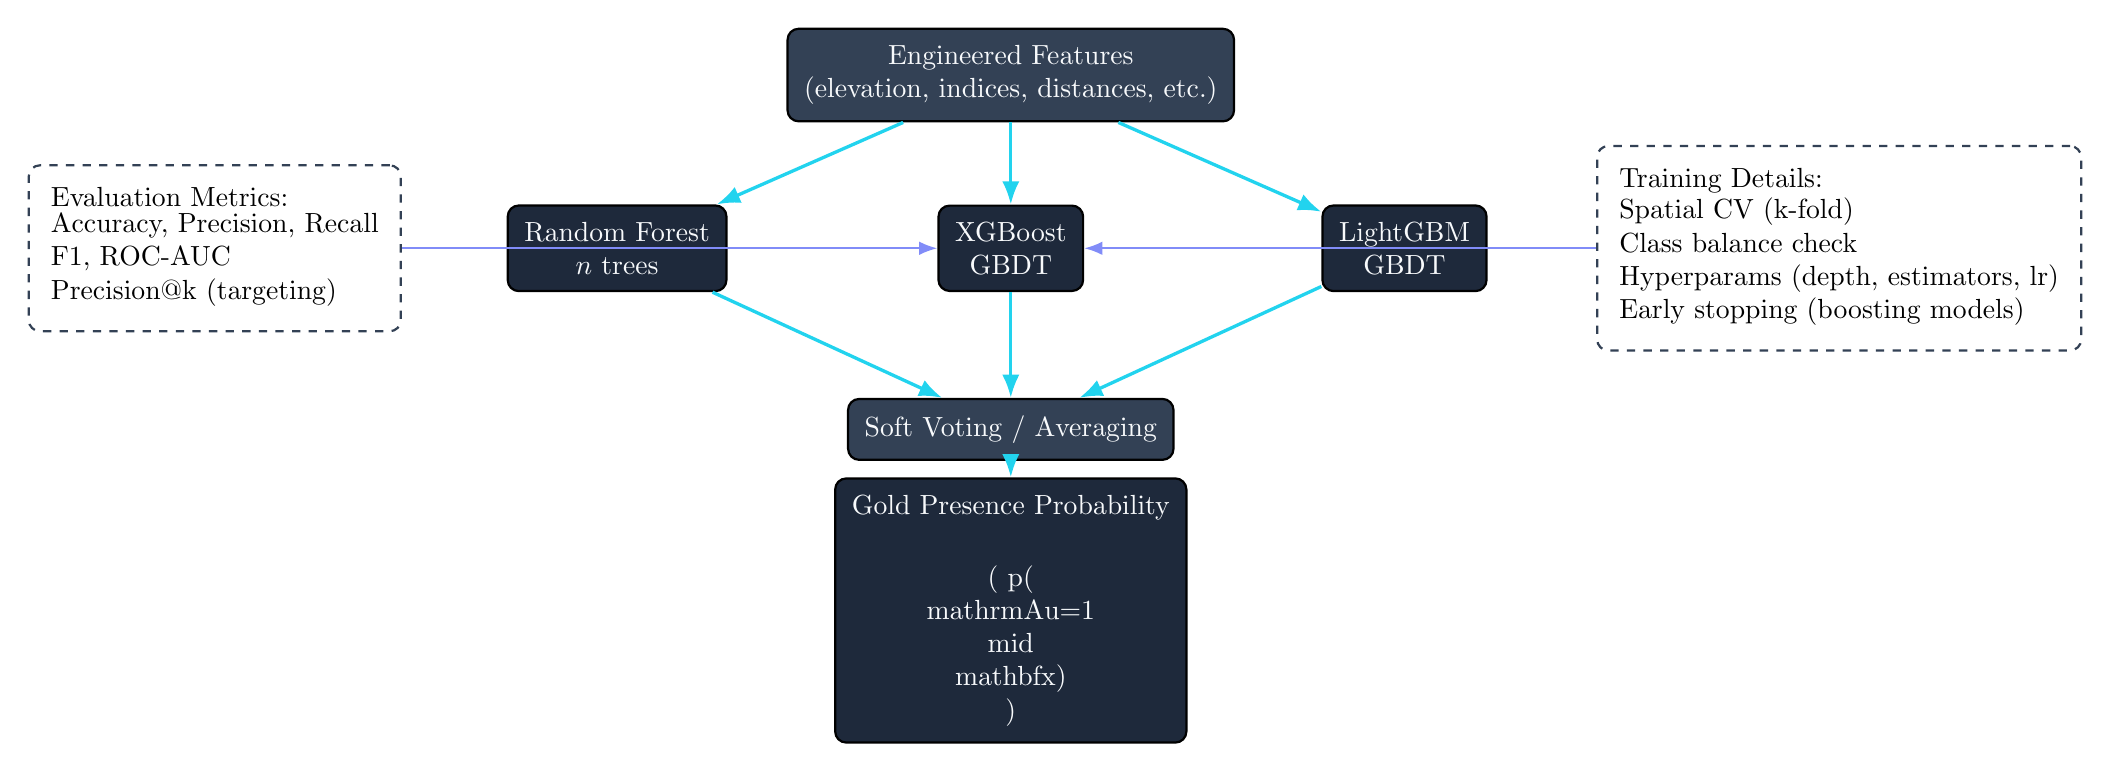
\begin{tikzpicture}[node distance=1.5cm]
  % Styles
  \tikzset{
    block/.style={draw, rounded corners, thick, align=center, fill=slate800, text=slate100, inner sep=6pt},
    data/.style={draw, rounded corners, thick, align=center, fill=slate700, text=slate100, inner sep=6pt},
    process/.style={draw, rounded corners, thick, align=center, fill=slate700, text=slate100, inner sep=6pt},
    result/.style={draw, rounded corners, thick, align=center, fill=slate800, text=slate100, inner sep=6pt},
    dashedblock/.style={draw=slate700, rounded corners, thick, align=center, dashed, inner sep=6pt},
    line/.style={-Latex, very thick, draw=cyan400},
    thinlink/.style={-Latex, thick, draw=indigo400},
  }

  % Inputs (fixed spacing)
  \node[data] (features) at (0,0) {Engineered Features\\(elevation, indices, distances, etc.)};

  % Base learners row
  \node[block] (rf)   at (-5,-2.2) {Random Forest\\$n$ trees};
  \node[block] (xgb)  at (0,-2.2)  {XGBoost\\GBDT};
  \node[block] (lgbm) at (5,-2.2)  {LightGBM\\GBDT};

  % Ensemble and output
  \node[process] (ens)  at (0,-4.5) {Soft Voting / Averaging};
  \node[result]  (proba) at (0,-6.8) {Gold Presence Probability\\[2pt] \\( p(\\mathrm{Au}=1\\mid \\mathbf{x}) \\)};

  % Links
  \draw[line] (features) -- (rf);
  \draw[line] (features) -- (xgb);
  \draw[line] (features) -- (lgbm);
  \draw[line] (rf) -- (ens);
  \draw[line] (xgb) -- (ens);
  \draw[line] (lgbm) -- (ens);
  \draw[line] (ens) -- (proba);

  % Side panels
  \node[dashedblock, right=6.5cm of xgb, align=left, inner sep=8pt] (trainbox) {Training Details:\\
    \begin{tabular}{@{}l@{}}
      Spatial CV (k-fold)\\
      Class balance check\\
      Hyperparams (depth, estimators, lr)\\
      Early stopping (boosting models)
    \end{tabular}
  };

  \node[dashedblock, left=6.8cm of xgb, align=left, inner sep=8pt] (evalbox) {Evaluation Metrics:\\
    \begin{tabular}{@{}l@{}}
      Accuracy, Precision, Recall\\
      F1, ROC-AUC\\
      Precision@k (targeting)
    \end{tabular}
  };

  \draw[thinlink] (trainbox.west) -- ++(-0.7,0) |- (xgb);
  \draw[thinlink] (evalbox.east) -- ++(0.7,0) |- (xgb);
\end{tikzpicture}
}
\end{frame}

\end{document}
\documentclass[aspectratio=169]{beamer}
\usetheme{Madrid}
\usepackage[utf8]{inputenc}
\usepackage{graphicx}
\usepackage{amsmath}
\usepackage{booktabs}
\usepackage{tikz}
\usetikzlibrary{arrows.meta,positioning,shapes,fit,calc}

% Title info
\title{GeoAuPredict: TikZ Diagrams}
\subtitle{Pipeline Flow and Model Architecture}
\author{GeoAuPredict Team}
\date{\today}

% TikZ styles
\tikzset{
  block/.style={draw, rounded corners, thick, align=center, fill=blue!10, inner sep=6pt},
  data/.style={draw, rounded corners, thick, align=center, fill=green!10, inner sep=6pt},
  process/.style={draw, rounded corners, thick, align=center, fill=orange!10, inner sep=6pt},
  result/.style={draw, rounded corners, thick, align=center, fill=purple!10, inner sep=6pt},
  dashedblock/.style={draw, rounded corners, thick, align=center, dashed, inner sep=6pt},
  line/.style={-Latex, very thick},
  thinlink/.style={-Latex, thick, gray},
}

\begin{document}

\frame{\titlepage}

% -------------------------------------------------
% Slide 1: End-to-end Pipeline Flow
% -------------------------------------------------
\begin{frame}{End-to-End Pipeline Flow}
\centering
\begin{tikzpicture}[node distance=1.6cm]
  % Row 1: Data sources
  \node[data] (geochem) {Geochemical\\Samples};
  \node[data, right=1.4cm of geochem] (terrain) {Terrain/DEM};
  \node[data, right=1.4cm of terrain] (remote) {Remote\\Sensing};
  \node[data, right=1.4cm of remote] (geology) {Geology\\Layers};

  % Row 2: Ingestion and preprocessing
  \node[process, below=1.4cm of $(geochem)!0.5!(terrain)$] (ingest) {Ingestion \& Preprocessing\\CRS align, resample, clip, clean};
  \node[process, below=1.4cm of $(remote)!0.5!(geology)$] (feat) {Feature Engineering\\indices, texture, distances};

  % Row 3: Split & CV
  \node[block, below=1.4cm of ingest] (split) {Spatial Train/Test Split\\(Geographic Blocks)};
  \node[block, below=1.4cm of feat] (cv) {Spatial Cross-Validation\\(k folds, geographic)};

  % Row 4: Models
  \node[block, below=1.6cm of $(split)!0.5!(cv)$, xshift=-3.0cm] (rf) {Random Forest};
  \node[block, below=1.6cm of $(split)!0.5!(cv)$] (xgb) {XGBoost};
  \node[block, below=1.6cm of $(split)!0.5!(cv)$, xshift=3.0cm] (lgbm) {LightGBM};

  % Row 5: Evaluation
  \node[result, below=1.6cm of $(rf)!0.5!(lgbm)$] (eval) {Evaluation\\Accuracy, F1, ROC-AUC, Precision@k};

  % Row 6: Mapping
  \node[result, below=1.6cm of eval] (mapping) {Probability Mapping\\(Kriging/Interpolation)};

  % Row 7: Deployment
  \node[result, below=1.6cm of mapping] (deploy) {Web/GIS Deployment\\Dashboards, APIs};

  % Connections: data to ingest
  \draw[line] (geochem) -- (ingest);
  \draw[line] (terrain) |- (ingest);
  \draw[line] (remote) |- (feat);
  \draw[line] (geology) -- (feat);

  % Ingest -> split, feat -> cv
  \draw[line] (ingest) -- (split);
  \draw[line] (feat) -- (cv);

  % Split/CV to models
  \draw[line] (split) |- (rf);
  \draw[line] (cv) -- (xgb);
  \draw[line] (split) |- (lgbm);

  % Models to evaluation
  \draw[line] (rf) -- (eval);
  \draw[line] (xgb) -- (eval);
  \draw[line] (lgbm) -- (eval);

  % Evaluation to mapping to deployment
  \draw[line] (eval) -- (mapping);
  \draw[line] (mapping) -- (deploy);

  % Group boxes
  \node[dashedblock, fit=(geochem) (terrain) (remote) (geology), label={[gray]above:Data Sources}] (dsbox) {};
  \node[dashedblock, fit=(ingest) (feat), label={[gray]above:Preparation}] (prepbox) {};
  \node[dashedblock, fit=(split) (cv), label={[gray]above:Validation Strategy}] (valbox) {};
  \node[dashedblock, fit=(rf) (xgb) (lgbm), label={[gray]above:Models}] (mdlbox) {};
  \node[dashedblock, fit=(eval) (mapping) (deploy), label={[gray]right:Outputs}] (outbox) {};
\end{tikzpicture}
\end{frame}

% -------------------------------------------------
% Slide 2: Model Architecture (Ensemble)
% -------------------------------------------------
\begin{frame}{Model Architecture: Ensemble for Gold Prediction}
\centering
\begin{tikzpicture}[node distance=1.5cm]
  % Inputs
  \node[data] (features) {Engineered Features\\(elevation, indices, distances, etc.)};

  % Base learners row
  \node[block, below=1.4cm of features, xshift=-4.2cm] (rf) {Random Forest\\$n$ trees};
  \node[block, below=1.4cm of features] (xgb) {XGBoost\\GBDT};
  \node[block, below=1.4cm of features, xshift=4.2cm] (lgbm) {LightGBM\\GBDT};

  % Ensemble
  \node[process, below=1.6cm of $(rf)!0.5!(lgbm)$] (ens) {Soft Voting / Averaging};

  % Output
  \node[result, below=1.6cm of ens] (proba) {Gold Presence Probability\\$p(\text{Au}=1\,|\,\mathbf{x})$};

  % Links
  \draw[line] (features) -- (rf);
  \draw[line] (features) -- (xgb);
  \draw[line] (features) -- (lgbm);

  \draw[line] (rf) -- (ens);
  \draw[line] (xgb) -- (ens);
  \draw[line] (lgbm) -- (ens);

  \draw[line] (ens) -- (proba);

  % Side panel: Training & Regularization
  \node[dashedblock, right=2.6cm of xgb, align=left, inner sep=8pt] (trainbox) {Training Details:\\
    \begin{tabular}{@{}l@{}}
      Spatial CV (k-fold)\\
      Class balance check\\
      Hyperparams (depth, estimators, lr)\\
      Early stopping (boosting models)
    \end{tabular}
  };

  % Side panel: Evaluation
  \node[dashedblock, left=2.8cm of xgb, align=left, inner sep=8pt] (evalbox) {Evaluation Metrics:\\
    \begin{tabular}{@{}l@{}}
      Accuracy, Precision, Recall\\
      F1, ROC-AUC\\
      Precision@k (targeting)
    \end{tabular}
  };

  % Thin links (context)
  \draw[thinlink] (trainbox.north west) |- (rf.east);
  \draw[thinlink] (trainbox) -- (xgb);
  \draw[thinlink] (trainbox.south west) |- (lgbm.east);

  \draw[thinlink] (evalbox.north east) |- (rf.west);
  \draw[thinlink] (evalbox) -- (xgb);
  \draw[thinlink] (evalbox.south east) |- (lgbm.west);
\end{tikzpicture}
\end{frame}

\end{document}

